In this chapter, we present our proposed methodology, including the methods and techniques used to address our research questions. We also cover our data exploration and preprocessing steps, the hyperparameter tuning process, and the automated and human evaluation methods and metrics we have chosen.

\subsection{Data exploration and preprocessing}
\subsubsection{Exploratory data analysis}

\subsubsection{Data preprocessing}

\subsubsection{Data augmentation}


\subsection{Automated evaluation metrics and baselines}
\subsubsection{Metrics}

\subsubsection{Baselines}
\todo{Write about baselines blabla}

\subsubsection{Automated evaluation pipeline}

\Cref{fig:data_pipeline} shows a flowchart of the automated evaluation pipeline, which contains the following sequential steps:

\begin{enumerate}

    \item \textbf{Data Fetching}: This is the first stage where dataset descriptions are downloaded from OpenML.

    \item \textbf{Data Preparation}: After fetching the data, the next step involves preparing it. This includes removing noise, correcting errors, augmenting it, and standardizing the format to prepare it for analysis. Data preparation ensures that the input to the topic model is of high quality, which is crucial for the success of the subsequent modeling steps. \\ The next step involves removing inadequate data points, such as excessively short descriptions and duplicates. Stop words are removed for models that require it (e.g., LDA). Additionally, the process includes stemming and lemmatization to normalize words to their base forms.

    \item \textbf{Topic Model}: In this step, the proposed topic model is applied to the prepared data. In this case, it will be BERTopic.

    \item \textbf{Benchmark Models}: Concurrently with the proposed topic model, benchmark models are run. These models represent established or baseline approaches to topic modeling against which the performance of the proposed topic model is compared. This will involve baseline models such as LDA, NMF and Top2Vec.

    \item \textbf{Topic Labels}: The output from both the topic model and the benchmark models are sets of topics, represented by a cluster of words that are characteristic of a particular topic.

    \item \textbf{Evaluation}: Finally, the performances of the proposed topic model and benchmark models are evaluated. This includes comparing the topic coherence and diversity.

\end{enumerate}

\begin{figure}[h]
    \centering
    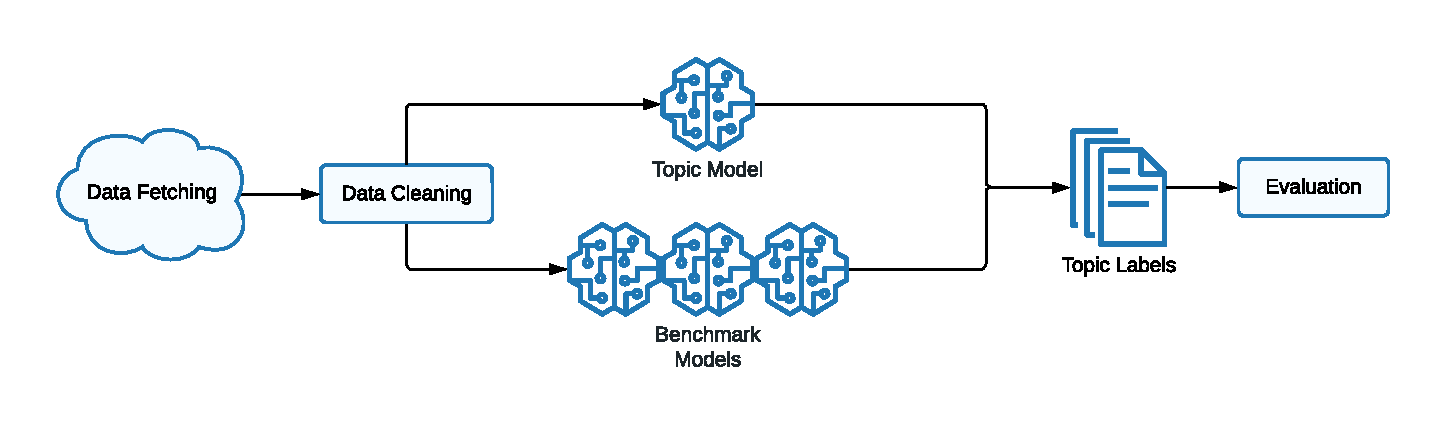
\includegraphics[width=\textwidth]{figures/data_pipeline.pdf}
    \caption{Data pipeline}
    \label{fig:data_pipeline}
\end{figure}

\subsubsection{Hyperparameter tuning}
\todo{Bayesian optimization...Refer back to \cref{fig:octis}}

\subsection{Tag generation}
In this subsection, we introduce our model, which is, in fact, a pipeline comprising multiple submodels and techniques. Steps 1-3 involve data preprocessing to prepare the data for the model. Steps 5-8 are referred to as the \textit{Base BERTopic model}, as these were optimized in the previous section on hyperparameter tuning and Bayesian optimization. Finally, steps 9 and 10 represent our improvements to the base model, introducing an approach that, to the best of our knowledge, is novel within the literature. Additionally, we provide an explanation of which steps are computationally efficient and which are more expensive.

\begin{figure}[h]
    \centering
    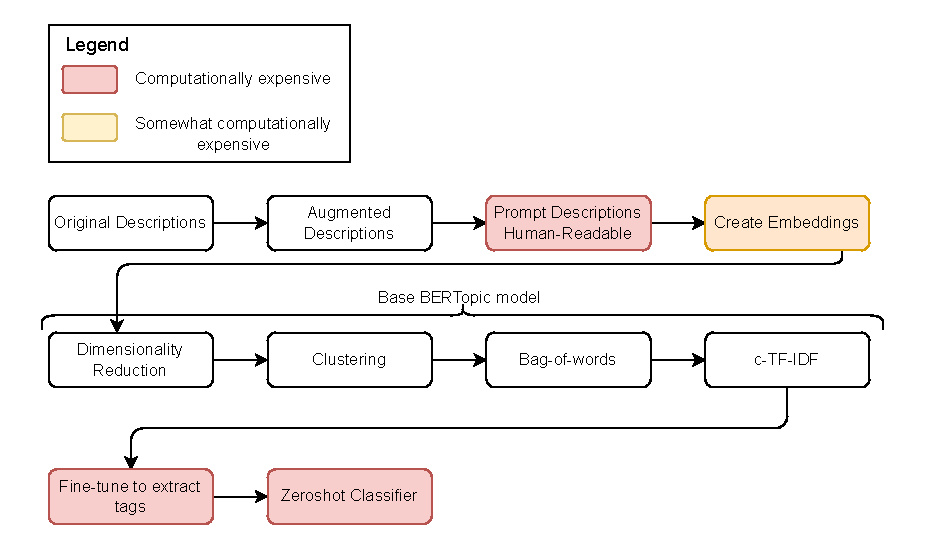
\includegraphics[width=\textwidth]{figures/tag_generation_pipeline.pdf}
    \caption{Tag generation pipeline}
    \label{fig:tag_generation_pipeline}
\end{figure}

To explain the pipeline illustrated in \cref{fig:tag_generation_pipeline} in more detail, we provide a step-by-step description of the process:

\begin{enumerate}
    \item \textbf{Original Descriptions}: The input to the pipeline is a set of original dataset descriptions. These come from the OpenML dataset and are used as the basis for generating tags.
    \item \textbf{Augmented Descriptions}: The OpenML dataset descriptions come with metadata such as dataset name, tags, features (column names) and some of them link to the original dataset, which can be used to scrape (extract) additional information. These are used to augment the dataset descriptions.
    \item \textbf{Prompt Descriptions Human Readable}: Augmented descriptions are rewritten to be more human readable via an LLM and prompt engineering. This is because the original descriptions are often in a technical format that is not easily interpretable by humans. Since LLMs are trained on large text corpora, they work best with human readable (natural language) text.
    \item \textbf{Create Embeddings}: Embeddings for each description are created using a pre-trained embedding model.
    \item \textbf{Dimensionality Reduction}: The dimensionality of the embeddings is reduced to cure the curse of dimensionality.
    \item \textbf{Clustering}: The reduced embeddings are clustered to group similar descriptions together. The output of this step is clusters, which represent our topics. Each cluster contains a set of descriptions (which we now call \textit{representative documents}) that are similar to each other.
    \item \textbf{Bag-of-words}: The descriptions in each cluster are converted to a bag-of-words representation, ignoring common words such as "the", "and", etc.
    \item \textbf{c-TF-IDF}: The bag-of-words representation is used to calculate the c-TF-IDF score for each word in each cluster. This score is used to rank the words in each cluster.
    \item \textbf{Fine-tune to extract tags}: For each topic, we have representative documents (from the clustering step) and representative words (from the c-TF-IDF step). We prompt engineer a question that asks an LLM to generate tags for each cluster. As context, we feed the LLM with the top \textit{k} representative documents and the top \textit{m} representative words for each topic. This results in tags that are common among the representative documents and representative words, and hence are representative of the topic.
    \item \textbf{Zeroshot Classifier}: Each description can in reality be contained in multiple clusters (topics). In this step, we get the top \textit{n} most likely clusters for each description. Then, for each description, we get the tags for each of the top \textit{n} clusters in a set. We feed this set of tags to a zeroshot text classification model, which returns confidences from 0 to 1 for whether each tag describes the description. This step is crucial for filtering out irrelevant tags for each description. For instance, if a description about diabetes and a description about cancer are both contained in the same topic (which may be, for example, "medical conditions"), we want to ensure that the tags for the cancer description are not assigned to the diabetes description. Furthermore, the description about diabetes may be contained in another topic that cancer is not in, such as "nutrition". In this case, we want to ensure that the tags in "nutrition" are not assigned to the cancer description, but are assigned to the diabetes description.

\end{enumerate}


\subsection{Human evaluation}
After designing our pipeline, we will perform a human evaluation to assess the quality of the tags produced by our model. As previously discussed, automated evaluation metrics offer only a limited perspective on the quality of the generated tags. Human evaluation is crucial for providing a more comprehensive assessment. To this end, we will carry out a user study in which participants will evaluate the quality of the tags generated by our model.

\subsubsection{Experimental design}
\paragraph{Participants}
We will begin by recruiting participants for the user study. Given that participants will be selected based on accessibility, this will constitute a convenience sample. Colleagues, friends, and acquaintances will be invited to participate. Despite the use of a convenience sample, we will aim to recruit individuals whose backgrounds align with those of OpenML's target users. Specifically, we will seek participants with expertise in data science, computer science, or, at a minimum, individuals with a bachelor's degree and a high proficiency in English.

\paragraph{Procedure}
\textbf{This section should describe how the experiment will be conducted. You could detail the steps participants will go through, such as how the tags will be presented to them, the instructions they will receive, and the criteria they are expected to evaluate.}

Participants will be presented with a set of items, each accompanied by tags generated by our model. They will be asked to evaluate the quality of the tags based on various criteria such as relevance, specificity, and clarity. Each tag will be rated on a Likert scale from 1 (poor quality) to 5 (excellent quality). Participants will also be given the option to provide qualitative feedback on the tags if they wish. The study will be conducted online, and participants will be given an estimated time to complete the evaluation.

\paragraph{Materials}
\textbf{This section outlines the tools, software, or datasets used in the study. In your case, this could include the interface for evaluating the tags, the source data, and the tags generated by the model.}

The evaluation interface will be a web-based platform, designed to present participants with items and their corresponding tags. The tags are generated by our model trained on the OpenML dataset. Each participant will be provided with a set of 20 items, with each item showing the tags generated by the model. The study will also include a brief tutorial on how to use the interface and what aspects of tag quality to focus on during evaluation.

\paragraph{Evaluation Criteria}
\textbf{This section defines the metrics or criteria that participants will use to evaluate the tags. This is crucial to ensure that the assessment is structured and focused on specific aspects of the tags' quality.}

Participants will evaluate the tags based on the following criteria:
\begin{itemize}
    \item \textbf{Relevance}: Do the tags accurately describe the content of the item?
    \item \textbf{Specificity}: Are the tags specific enough to distinguish between similar items?
    \item \textbf{Clarity}: Are the tags easy to understand and unambiguous?
    \item \textbf{Usefulness}: Would these tags help a user searching for similar content?
\end{itemize}
Each criterion will be rated on a 5-point Likert scale, with space for additional comments.

\paragraph{Data Collection}
During the evaluation, participants' ratings and feedback will be automatically recorded through the web interface. All data will be anonymized and stored in a secure database. No personally identifiable information will be collected, and participants will be assigned a unique ID to keep their responses anonymous. The collected data will include numerical ratings for each criterion as well as any optional qualitative feedback provided by participants.

\paragraph{Analysis Plan}
The quantitative data from the Likert-scale ratings will be analyzed using descriptive statistics, such as means and standard deviations for each criterion. Additionally, we will conduct statistical tests (e.g., a t-test or ANOVA) to determine if there are significant differences in tag quality across different items. Qualitative feedback will be analyzed using thematic analysis to identify common themes in participants' perceptions of tag quality. This will help us understand not only the numerical ratings but also the reasons behind participants' judgments.

\paragraph{Ethical Considerations}
All participants will be required to provide informed consent before taking part in the study. They will be informed about the purpose of the study, what their participation entails, and how their data will be used. Participants will have the right to withdraw from the study at any time without any consequences. All data collected will be anonymized, and no personally identifiable information will be stored. The study protocol has been reviewed and approved by the appropriate ethics review board.

\paragraph{Limitations}
\textbf{This section acknowledges any potential limitations of your experimental design, such as the use of a convenience sample or the limited generalizability of the results.}

One limitation of this study is the use of a convenience sample, which may not be fully representative of the target user base of OpenML. While we aim to recruit participants with relevant backgrounds, the results may still be subject to selection bias. Additionally, the subjective nature of human evaluation means that individual biases and preferences could affect the results. To mitigate this, we will aim to recruit a diverse group of participants and analyze the data for any potential biases.

\paragraph{Hypotheses}
We hypothesize that the tags generated by our model will score highly on relevance and clarity but may need improvement in specificity. We also expect that participants with a stronger background in data science will provide more critical feedback compared to those with less technical expertise.